\begin{flushleft}
La funzione data è \[F(x_1, x_2)= \begin{cases}x_2-cos(x_1)\\ x_1x_2 -1/2\end{cases}\]
Vogliamo trovare $F(x_1, x_2)=0$ partendo da $x_1(0) = 1\mbox{, } x_2(0) = 1$\\
Troviamo quindi il Jacobiano della funzione: 
\[ 
J=\begin{pmatrix} sin(x_1) & 1  \\\ x_1 & x_2 \end{pmatrix}
\]
Applicando il metodo di Newton si va a risolvere:
\[
\begin{cases} 
J_F(\underline{x}^{(k)})\underline{d}^{(k)}=-F(\underline{x}^{(k)}) \\ 
\quad \underline{x}^{(k+1)}=\underline{x}^{(k)}+\underline{d}^{(k)} 
\end{cases}
\]
Usando il codice MatLab:
\lstinputlisting[language=Matlab]{cap_3/es20/es20.m}
si ottengono i risultati:
\begin{figure}[h]
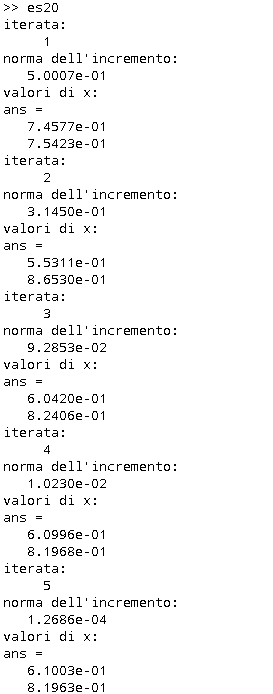
\includegraphics[left, width=320px, height=400px]{cap_3/es20/es320}
\end{figure}
\newline \\
Che in forma tabellare sono rappresentati da:
\begin{center}
\begin{tabular}{|l|c|c|c|}
\hline
i & $x_1$ & $x_2$ & Norma incremento \\
\hline
1 & 0.7458 & 0.7542 & 0.50007 \\
2 & 0.5531 & 0.8653 & 0.31450 \\
3 & 0.6042 & 0.8241 & 0.09285 \\
4 & 0.6100 & 0.8197 & 0.01023 \\
5 & 0.6100 & 0.8196 & 0.00013 \\ 
\hline
\end{tabular}
\end{center}
\end{flushleft}